\subsection{\label{sub:\projectname-regs} \textsf{regs}}

\paragraph{Símbol}

\begin{center} \bsfsymbol{regs} \end{center}

\paragraph{Entrades i sortides}

\begin{where}
\item[\nodenamebit{intro}] Senyal que s'activa si s'ha d'emmagatzemar una xifra nova
\item[\nodenamerange{keycode}{3}{0}] Xifra que s'està introduint (BCD)
\item[\nodenamerange{opA}{3}{0}] Primera xifra desada (BCD)
\item[\nodenamerange{opB}{3}{0}] Segona xifra desada (BCD)
\item[\nodenamebit{clk}] Rellotge, flanc de pujada
\item[\nodenamebit{nrst}] Reset asíncron, actiu baix
\end{where}

\paragraph{Funció}

Registres per als factors.

Emmagatzema les xifres premudes en dos registres per a $opA$ i $opB$.
Inicialment ambdós son zero; quan $intro$ és actiu, la xifra a l'entrada $keycode$
s'emmagatzema a $opA$ i el valor anterior de $opA$ s'emmagatzema a $opB$.

\paragraph{Inespecificacions}

Cap.

\paragraph{Implementació}

\begin{contendfig}
  \begin{center}
    \adjustbox{max width=\textwidth, max height=\textheight}{
      \bdfschematic{regs}
    }
  \end{center}
  \caption{\label{fig:sch-\projectname-regs} Esquemàtic per al bloc \textsf{regs}}
\end{contendfig}

L'esquemàtic del bloc es pot veure a la figura~\ref{fig:sch-\projectname-regs} (pàgina~\pageref{fig:sch-\projectname-regs}).

Dos biestables D amb habilitació de càrrega encadenats, de forma similar a un \emph{shift
register}. Les sortides dels biestables es retornen en ordre a $opA$ i $opB$.

\paragraph{Simulació}

\begin{contendfig}
  \begin{center}
    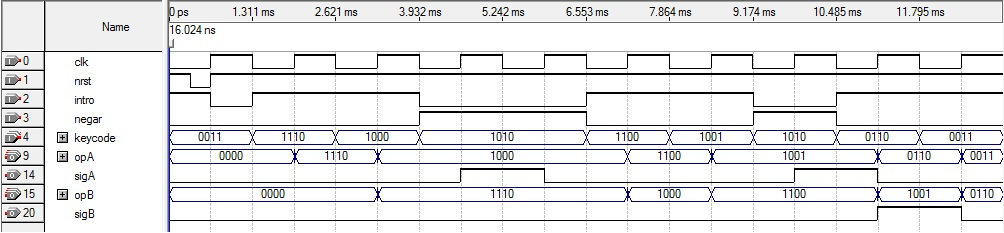
\includegraphics[scale=0.55]{../\projectname/assets/vwf/regs.jpg}
  \end{center}
  \caption{\label{fig:sim-\projectname-regs} Simulació per al bloc \textsf{regs}}
\end{contendfig}

La simulació del bloc es pot veure a la figura~\ref{fig:sim-\projectname-regs} (pàgina~\pageref{fig:sim-\projectname-regs}).

% FIXME

\vspace{1cm}
